\begin{frame}{Scientific context}
	\begin{minipage}{0.75\linewidth}
		\textbf{Context :} Create real-time digital twins of an organ (e.g. liver).
	\end{minipage}
	\begin{minipage}{0.21\linewidth}
		\vspace{-20pt}
		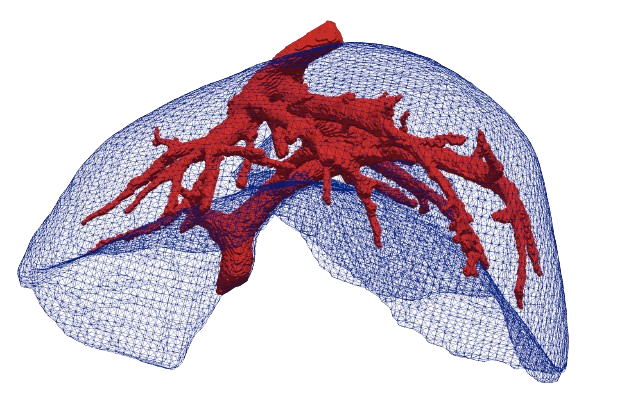
\includegraphics[width=\linewidth]{images/intro/liver.png}
	\end{minipage}
	
	\vspace{5pt}
	\textbf{Objective :} Develop an hybrid \fcolorbox{red}{white}{finite element} / \fcolorbox{orange}{white}{neural network} method.
	
	\vspace{1pt}
	\small
	\hspace{130pt} \begin{minipage}{0.14\linewidth}
		\textcolor{red}{accurate}
	\end{minipage} \hspace{8pt} \begin{minipage}{0.3\linewidth}
		\textcolor{orange}{quick + parameterized}
	\end{minipage}

	\begin{figure}[!ht]
		\centering
		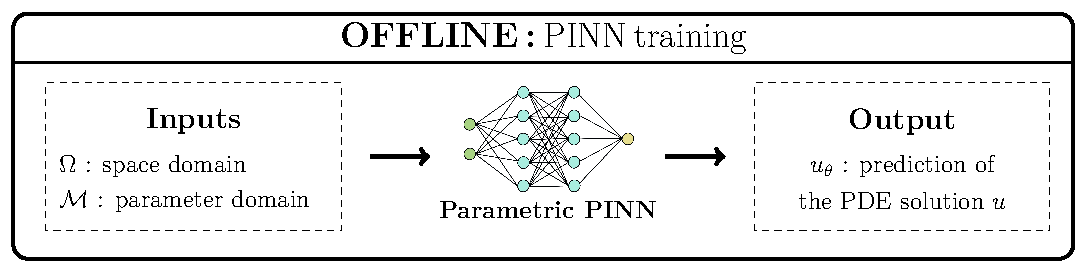
\includegraphics[width=0.7\linewidth]{images/intro/pipeline/offline.pdf}

		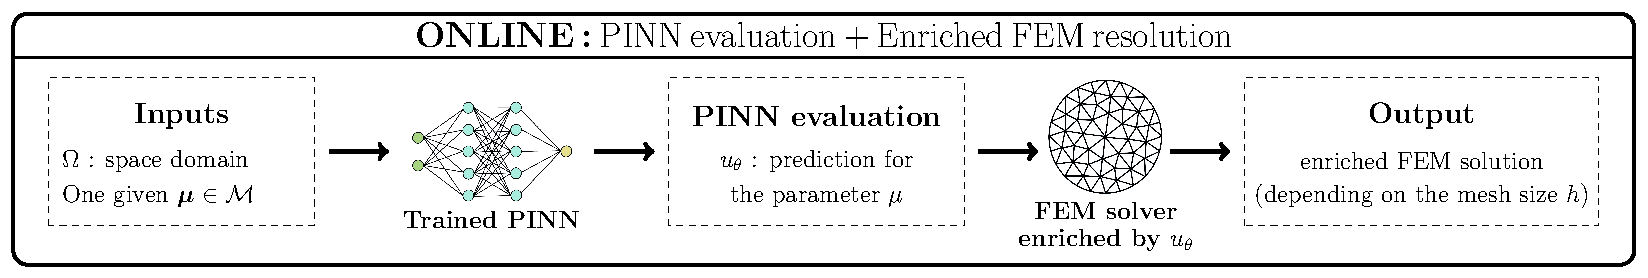
\includegraphics[width=\linewidth]{images/intro/pipeline/online.pdf}
	\end{figure}
\end{frame}

\begin{frame}{Problem considered}
	\only<2-3>{\textcolor{red}{\textbf{Objective:} Simulate the flow for a range of $\bm{\mu} = (\mu,k_f) \in \mathcal{M} = [0.01, 0.1]^2$.}
	
	\vspace{5pt}}

	\textbf{Stationary incompressible Navier-Stokes equations (with buoyancy and gravity) :}

	We consider \only<1>{$\Omega = [-1,1]^2$ a squared domain}\only<2-3>{\textcolor{red}{$\bm{x}=(x,y)\in\Omega$}} and $\bm{e}_y = (0,1)$.
	
	Find \only<1>{the velocity $\bm{u}=(u,v)$, the pressure $p$ and the temperature $T$}\only<2-3>{\textcolor{red}{$\bm{U} = (\bm{u},p,T) = (u,v,p,T)$}} such that
	\begin{equation} \label{eq:Pb}
		\left\{\begin{aligned}
			&\only<1>{(\bm{u} \cdot \nabla)\bm{u} + \nabla p - \mu \Delta \bm{u} - g (\beta T + 1)\bm{e}_y}\only<2-3>{\textcolor{red}{R_{mom}(U;\bm{x},\bm{\mu})}} = 0 \;\; \text{in } \Omega \quad &&\text{\small (momentum)} \\
			&\only<1>{\nabla \cdot \bm{u}}\only<2-3>{\textcolor{red}{R_{inc}(U;\bm{x},\bm{\mu})}} = 0 \;\; \text{in } \Omega \quad &&\text{\small (incompressibility)} \\
			&\only<1>{\bm{u} \cdot \nabla T - k_f \Delta T}\only<2-3>{\textcolor{red}{R_{ener}(U;\bm{x},\bm{\mu})}} = 0 \;\; \text{in } \Omega \quad &&\text{\small (energy)} \only<1-2>{\\
			&\text{+ suitable BC}}
		\end{aligned}\right.
		\tag{$\mathcal{P}$}
	\end{equation}
	
	with $g=9.81$ the gravity, $\beta=0.1$ the expansion coefficient, $\mu$ the viscosity and $k_f$ the thermal conductivity. \citep{coulaud_investigations_2024}

	\vspace{5pt}

	\only<3>{\textbf{Boundary Conditions:} 

	\begin{itemize}
		\item $\bm{u} = 0$ on $\partial\Omega$
		\item $T = 1$ on the left wall ($x=-1$) and $T = -1$ on the right wall ($x=1$) \\
		$\displaystyle \frac{\partial T}{\partial n} = 0$ on the top and bottom walls ($y=\pm 1$)	
	\end{itemize}}

\end{frame}